\documentclass[tikz,border=6pt]{standalone}
\usepackage{amsmath,amssymb}
\usetikzlibrary{arrows.meta}
\begin{document}
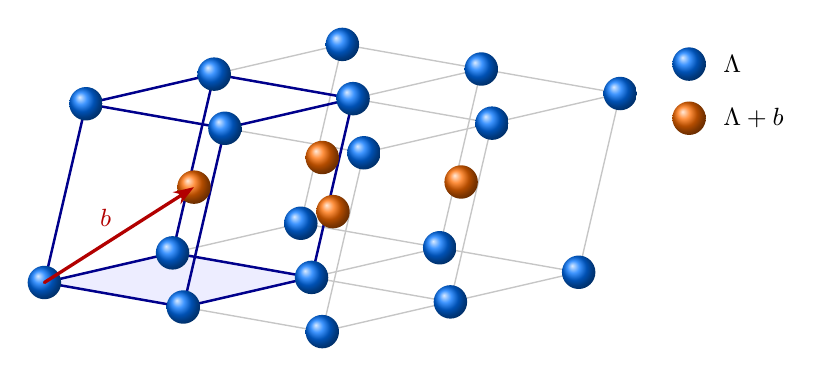
\begin{tikzpicture}[scale=1.25,line cap=round,>={Stealth[length=2.6mm,width=1.8mm]}]
  % the fundamental cell spanned by a basis of the lattice
  \fill[blue!7] (0.000,0.000)--(1.302,0.301)--(2.714,0.052)--(1.411,-0.249)--cycle;
  % the cells of the lattice, behind the points
  \draw[gray!45,line width=0.5pt] (0.000,0.000)--(1.302,0.301);
  \draw[gray!45,line width=0.5pt] (0.000,0.000)--(1.411,-0.249);
  \draw[gray!45,line width=0.5pt] (0.000,0.000)--(0.423,1.816);
  \draw[gray!45,line width=0.5pt] (0.423,1.816)--(1.725,2.117);
  \draw[gray!45,line width=0.5pt] (0.423,1.816)--(1.834,1.567);
  \draw[gray!45,line width=0.5pt] (1.411,-0.249)--(2.714,0.052);
  \draw[gray!45,line width=0.5pt] (1.411,-0.249)--(2.823,-0.499);
  \draw[gray!45,line width=0.5pt] (1.411,-0.249)--(1.834,1.567);
  \draw[gray!45,line width=0.5pt] (1.834,1.567)--(3.136,1.868);
  \draw[gray!45,line width=0.5pt] (1.834,1.567)--(3.246,1.318);
  \draw[gray!45,line width=0.5pt] (2.823,-0.499)--(4.125,-0.197);
  \draw[gray!45,line width=0.5pt] (2.823,-0.499)--(3.246,1.318);
  \draw[gray!45,line width=0.5pt] (3.246,1.318)--(4.548,1.619);
  \draw[gray!45,line width=0.5pt] (1.302,0.301)--(2.605,0.602);
  \draw[gray!45,line width=0.5pt] (1.302,0.301)--(2.714,0.052);
  \draw[gray!45,line width=0.5pt] (1.302,0.301)--(1.725,2.117);
  \draw[gray!45,line width=0.5pt] (1.725,2.117)--(3.027,2.419);
  \draw[gray!45,line width=0.5pt] (1.725,2.117)--(3.136,1.868);
  \draw[gray!45,line width=0.5pt] (2.714,0.052)--(4.016,0.353);
  \draw[gray!45,line width=0.5pt] (2.714,0.052)--(4.125,-0.197);
  \draw[gray!45,line width=0.5pt] (2.714,0.052)--(3.136,1.868);
  \draw[gray!45,line width=0.5pt] (3.136,1.868)--(4.439,2.169);
  \draw[gray!45,line width=0.5pt] (3.136,1.868)--(4.548,1.619);
  \draw[gray!45,line width=0.5pt] (4.125,-0.197)--(5.428,0.104);
  \draw[gray!45,line width=0.5pt] (4.125,-0.197)--(4.548,1.619);
  \draw[gray!45,line width=0.5pt] (4.548,1.619)--(5.850,1.920);
  \draw[gray!45,line width=0.5pt] (2.605,0.602)--(4.016,0.353);
  \draw[gray!45,line width=0.5pt] (2.605,0.602)--(3.027,2.419);
  \draw[gray!45,line width=0.5pt] (3.027,2.419)--(4.439,2.169);
  \draw[gray!45,line width=0.5pt] (4.016,0.353)--(5.428,0.104);
  \draw[gray!45,line width=0.5pt] (4.016,0.353)--(4.439,2.169);
  \draw[gray!45,line width=0.5pt] (4.439,2.169)--(5.850,1.920);
  \draw[gray!45,line width=0.5pt] (5.428,0.104)--(5.850,1.920);
  \draw[blue!55!black,line width=0.9pt] (0.000,0.000)--(0.423,1.816);
  \draw[blue!55!black,line width=0.9pt] (0.000,0.000)--(1.411,-0.249);
  \draw[blue!55!black,line width=0.9pt] (0.000,0.000)--(1.302,0.301);
  \draw[blue!55!black,line width=0.9pt] (0.423,1.816)--(1.834,1.567);
  \draw[blue!55!black,line width=0.9pt] (0.423,1.816)--(1.725,2.117);
  \draw[blue!55!black,line width=0.9pt] (1.411,-0.249)--(1.834,1.567);
  \draw[blue!55!black,line width=0.9pt] (1.411,-0.249)--(2.714,0.052);
  \draw[blue!55!black,line width=0.9pt] (1.834,1.567)--(3.136,1.868);
  \draw[blue!55!black,line width=0.9pt] (1.302,0.301)--(1.725,2.117);
  \draw[blue!55!black,line width=0.9pt] (1.302,0.301)--(2.714,0.052);
  \draw[blue!55!black,line width=0.9pt] (1.725,2.117)--(3.136,1.868);
  \draw[blue!55!black,line width=0.9pt] (2.714,0.052)--(3.136,1.868);
  % the points, from back to front
  \shade[ball color=blue!55!cyan] (3.246,1.318) circle (0.17);
  \shade[ball color=blue!55!cyan] (2.823,-0.499) circle (0.17);
  \shade[ball color=blue!55!cyan] (1.834,1.567) circle (0.17);
  \shade[ball color=blue!55!cyan] (4.548,1.619) circle (0.17);
  \shade[ball color=orange!85!red] (2.932,0.720) circle (0.17);
  \shade[ball color=blue!55!cyan] (1.411,-0.249) circle (0.17);
  \shade[ball color=blue!55!cyan] (4.125,-0.197) circle (0.17);
  \shade[ball color=blue!55!cyan] (0.423,1.816) circle (0.17);
  \shade[ball color=blue!55!cyan] (3.136,1.868) circle (0.17);
  \shade[ball color=blue!55!cyan] (5.850,1.920) circle (0.17);
  \shade[ball color=orange!85!red] (1.520,0.969) circle (0.17);
  \shade[ball color=blue!55!cyan] (0.000,0.000) circle (0.17);
  \shade[ball color=orange!85!red] (4.234,1.021) circle (0.17);
  \shade[ball color=blue!55!cyan] (2.714,0.052) circle (0.17);
  \shade[ball color=blue!55!cyan] (5.428,0.104) circle (0.17);
  \shade[ball color=blue!55!cyan] (1.725,2.117) circle (0.17);
  \shade[ball color=blue!55!cyan] (4.439,2.169) circle (0.17);
  \shade[ball color=orange!85!red] (2.823,1.270) circle (0.17);
  \shade[ball color=blue!55!cyan] (1.302,0.301) circle (0.17);
  \shade[ball color=blue!55!cyan] (4.016,0.353) circle (0.17);
  \shade[ball color=blue!55!cyan] (3.027,2.419) circle (0.17);
  \shade[ball color=blue!55!cyan] (2.605,0.602) circle (0.17);
  \draw[->,very thick,red!70!black] (0.000,0.000)--(1.520,0.969) node[midway,above left=-1pt,font=\small] {$b$};
  \shade[ball color=blue!55!cyan] (6.550,2.219) circle (0.17); \node[right,font=\small] at (6.800,2.219) {$\Lambda$};
  \shade[ball color=orange!85!red] (6.550,1.669) circle (0.17); \node[right,font=\small] at (6.800,1.669) {$\Lambda+b$};
\end{tikzpicture}
\end{document}
